\documentclass{sig-alternate}

\usepackage{url}
\usepackage{amsmath}
\usepackage{graphicx}
\usepackage{subfigure}
\usepackage{threeparttable}
\usepackage{pdflscape}
\usepackage{array}
\usepackage{color}

\begin{document}

\title{The Bug Catalog of the Maven Repository Ecosystem}

\numberofauthors{5} 

\author{
% 1st. author
\alignauthor
Dimitris Mitropoulos\\
       \affaddr{Athens University of Economics and Business}\\
       \affaddr{Department of Management Science and Technology}\\
       \email{dimitro@aueb.gr}
% 2nd. author
\alignauthor Vassilios Karakoidas\\
       \affaddr{Athens University of Economics and Business}\\
       \affaddr{Department of Management Science and Technology}\\
       \email{bkarak@aueb.gr}
% 3rd. author
\alignauthor Panos Louridas\\
       \affaddr{Athens University of Economics and Business}\\
       \affaddr{Department of Management Science and Technology}\\
       \email{louridas@aueb.gr}
\and  % use '\and' if you need 'another row' of author names
% 4th. author
\alignauthor Georgios Gousios\\
       \affaddr{Delft University of Technology}\\
       \affaddr{Software Engineering Research Group}\\
       \email{G.Gousios@tudelft.nl}
% 5th. author
\alignauthor Diomidis Spinellis\\
       \affaddr{Athens University of Economics and Business}\\
       \affaddr{Department of Management Science and Technology}\\
       \email{dds@aueb.gr}
}

\maketitle
\begin{abstract}
Examining software ecosystems can provide the research community
with useful information. To examine the Maven Central Repository
(approximately 265{\sc gb} of data), we performed an experiment
where we statically analyzed the repository to detect its software
bugs. For our analysis we used FindBugs, a tool that
examines Java bytecode to detect numerous types of bugs.
In this paper, we present our data collection experiment
and show how our dataset can be used to extract interesting
findings on software evolution.
\end{abstract}

\category{D.2.4}{Software Engineering}{Software/Program Verification}[Statistical methods]
\category{D.2.5}{Software Engineering}{Testing and Debugging}[Code inspections and walk-throughs]
\category{D.2.7}{Software Engineering}{Distribution, Maintenance, and Enhancement}[Version control]

\terms{Static Analysis, Software Ecosystems}

\keywords{Maven Repository, FindBugs, Software Bugs}

\section{Introduction}
\label{sec:intro}

A software ecosystem can be seen as a collection of software projects,
which are developed and co-evolve in the same environment~\cite{LL10}.
Components can be interdependent and have multiple versions.
Examples of such ecosystems include Python's
{\sc p}y{\sc py}\footnote{\url{http://pypy.org/}}
(Python Package Index), Perl's
{\sc cpan}\footnote{\url{http://www.cpan.org/}}
(Comprehensive Perl Archive Network), Ruby's
RubyGems\footnote{\url{http://rubygems.org/}}
and the Maven Central Repository.\footnote{\url{http://mvnrepository.com/}}

Maven is a build automation tool used primarily for Java projects and it is
hosted by the Apache Software Foundation.
It uses {\sc xml} to describe the software project being built, its dependencies
on other external modules, the build order, and required plug-ins.
To build a software component, it dynamically downloads Java libraries
and Maven plug-ins from the Maven central repository,
and stores them in a local cache. The repository can be updated with
new projects and also with new versions of existing projects
that can depend on other versions.

To statically analyze the Maven repository
we used {\it FindBugs},\footnote{\url{http://findbugs.sourceforge.net/}}
a static analysis tool that examines bytecode to detect software bugs
and has already been used in research~\cite{AP10,SHP06}.
Specifically, we ran FindBugs on all the project versions of all
the projects that exist in the repository
to identify all bugs contained in it.

In this paper we present: a) the experiment performed to obtain the
collection of the metric results that the FindBugs tool produces and
b) how researchers can actually use the dataset and include it in
their research.

\section{Data Collection Experiment}
\label{sec:exp}
Body.

\section{Repository Statistics}
\label{sec:repo}
Repo stats.

\begin{figure}[t]
	\centering
	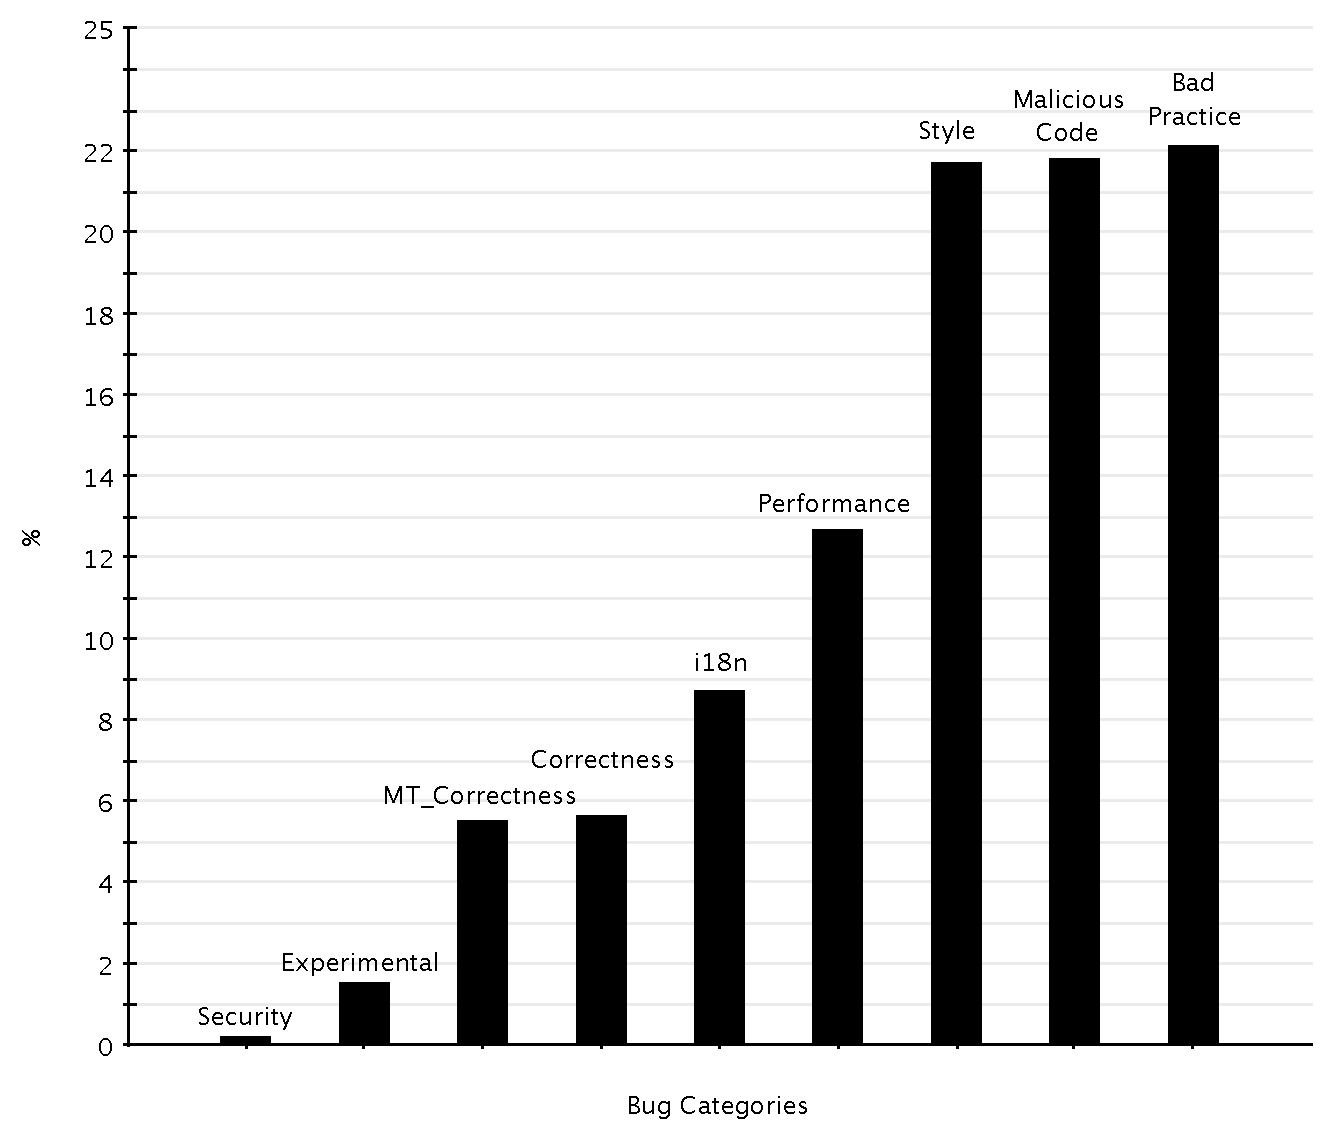
\includegraphics[scale=0.38]{figures/bug_percent}
	\caption{Bug percentage in Maven repository.}
	\label{fig:bug-per} 
\end{figure}

\section{Initial Findings}
\label{sec:find}
Findings.

\section{Tools}
\label{sec:exp}
Tools.

\section{Related Work}
\label{sec:rel}

Cite~\cite{RDV13}.

\section{Conclusions}
\label{sec:conc}

\section{Acknowledgments}
possible acks.

\bibliographystyle{abbrv}
\bibliography{msr}  
\end{document}
